%%
%% Template intro.tex
%%

\chapter{Introduction}
\label{cha:intro}

Given the vast amount of content available on the Internet, finding
information of personal interest (news, blogs, videos, movies, books,
etc.) is often like finding a needle in a haystack.  Recommender
systems based on \emph{collaborative filtering} (CF) aim to address
this problem by leveraging the preferences of a user
population under the assumption that similar users
will have similar preferences.  These principles underlie the
recommendation algorithms powering websites like Amazon and
Netflix.\footnote{On Amazon, this is directly evident with statements
displayed of the form ``users who looked at item X ended up purchasing
item Y 90\% of the time''.  While the exact inner workings of Netflix
are not published, the best performing recommendation algorithm in
the popular Netflix prize competition~\cite{netflix} 
used an ensemble of CF methods.}

As the web has become more social with the emergence of Facebook,
Twitter, LinkedIn, and most recently Google+, this adds myriad new
dimensions to the recommendation problem by making available a rich
labeled graph structure of social content from which user preferences
can be learned and new recommendations can be made.  In this socially
connected setting, no longer are web users simply described by an IP
address (with perhaps associated geographical information and browsing
history), but rather they are described by a rich user profile (age,
gender, location, educational and work history, preferences, etc.)
and a rich history of user interactions with their friends (comments/posts, 
clicks of like, tagging in photos, mutual group
memberships, etc.).  This rich information poses both an amazing
opportunity and a daunting challenge for machine learning methods
applied to social recommendation --- how do we fully exploit the social
network content in recommendation algorithms?

\section{Objectives}

%%%%%%%%%%%%%%%%%%%%%%%%%%%%%%%%%%%%%%%%%%%%%%%%%%%%%%%%%%%%%
\begin{figure}[t!]
\centering
%\subfigure{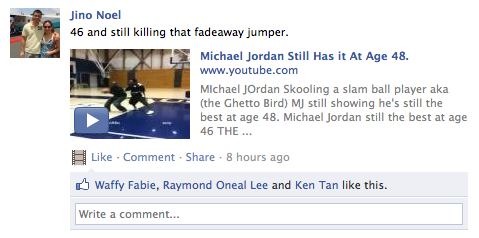
\includegraphics[scale=0.50]{img/posted-link.png}}
\subfigure{
\includegraphics[scale=0.85]{img/posted-link.eps}}
\caption{A link posted by the author that has been liked by three
other users.  The objective of this thesis is to build an automated
link recommendation App for Facebook that learns user preferences
via social collaborative filtering techniques 
and automatically recommends links (such as this one) to other users.
We actively collect like/dislike feedback from the users to measure
recommendation algorithm performance and to learn from for future
recommendations.}
\label{fig:ex_link}
\end{figure}
%%%%%%%%%%%%%%%%%%%%%%%%%%%%%%%%%%%%%%%%%%%%%%%%%%%%%%%%%%%%%

This thesis examines the problem of designing efficient, scalable, and
accurate \emph{social CF} (SCF) algorithms for \emph{personalized link
recommendation on Facebook} -- quite simply the task of recommending
personalized links to users that might interest them.  We show an
example link posted on Facebook in Figure~\ref{fig:ex_link} that we
might wish to recommend to a subset of users; once link recommendations
such as this one are made, we then need to gather 
feedback from users in order to (a) learn to make better
recommendations in the future and (b) to evaluate the
efficacy of our different recommendation approaches.  
%\emph{User
%interest} can be determined via many methods including \emph{indirect
%feedback} in the form of link clicks and \emph{direct feedback} in the
%form of explicit link ratings or other evidence that a user
%\emph{liked} a link (e.g., explicitly clicking ``like'').

Many existing SCF approaches that can be applied to recommendation
tasks like this one extend \emph{matrix
factorization} (MF) techniques~\cite{pmf} and have proved quite
powerful in their ability to accurately model user preferences even
when only a unique ID is available for both the user and item being
recommended.  The power of such methods stems from their ability to
project users and items into latent vector spaces of reduced
dimensionality where each is effectively grouped by similarity.
Indeed, we will show in Chapter 4 that existing social extensions of
MF are quite powerful and outperform a variety of other commonly used
SCF approaches.

Given the strong performance of existing MF approaches to SCF, we aim
to comparatively evaluate them and further improve on their
performance when applied to link recommendation on Facebook.  
To do this, we first identify a number of
major deficiencies of existing SCF MF methods that we make our objective to
address in this thesis:
\begin{enumerate}
\item[(a)] {\bf Non-feature-based user similarity:} Existing SCF MF
methods do not permit the use of item or link features in learning
user similarity based on observed interactions.  For example, 
the fact that two users have the same gender cannot be exploited
by existing methods SCF MF methods that make use of user similarity.
% Note: potential for latent item information diffusion here
\item[(b)] {\bf Model direct user-user information diffusion:}
Existing SCF MF methods do not permit directly modeling user-user
information diffusion according to the social graph structure.  For example,
if a certain user always likes content from another specific user,
this simply cannot be learned by existing SCF MF methods.
\item[(c)] {\bf Restricted common interests:} Existing SCF MF methods
cannot learn from the fact that two users have common overlapping interests
in specific areas.  For example, a friend and their co-worker may
both like the same links regarding technical content, but have differing
interests when it comes to politically-oriented links --- knowing this
would allow one to recommend technical content posted by one user to the
other, but existing SCF methods cannot explicitly encourage this.
\end{enumerate}

This thesis addresses all of these problems with novel contributions in
an efficient, scalable, and unified latent factorization component
framework for SCF.  We present results of our algorithms on live
trials in a custom-developed Facebook App involving data collected
over three months from over 100 App users and their nearly 30,000
friends.  These results show that a number of extensions proposed to
resolve (a)--(c) outperform all previously existing algorithms.

In addition, given that live online user evaluation trials are
time-consuming, requiring many users and often an evaluation period of
at least one month, we have one last important objective to address in
this thesis:
\begin{enumerate}
\item[(d)] {\bf Idenfying passive evaluation paradigms that correlate
with actively elicited human judgments.}  The benefits of doing this
are many-fold.  When designing new SCF algorithms, there are myriad
design choices to be made, for which actual performance evaluation is
the only way to validate the correct choice.  Furthermore, simple
parameter tuning is crucial for best performance and SCF algorithms
are often highly sensitive to well-tuned parameters.  Thus for the
purpose of algorithm design and tuning, it is crucial to have methods
and metrics that can be evaluated immediately on passive data (i.e., a
passive data set of user likes) that are shown to correlate with human
judgments in order to avoid the time-consuming process of evaluating
the algorithms in live human trials.
\end{enumerate}

%Having defined these problem objectives to focus on, 
%next we outline our specific thesis contributions to address these problems.

\section{Contributions}

\label{sec:Contributions}

In the preceding section, we outlined three deficiencies of existing MF
approaches for SCF.  Now we discuss our specific
contributions in this thesis to address these three deficiencies:
\begin{enumerate}
\item[(a)] {\bf User-feature social regularization:} One can encode
prior knowledge into the learning process using a technique known as
\emph{regularization}.  In the case of social MF, we often want to
regularize the learned latent representations of users to enforce that
users who interact heavily often have similar preferences, and hence
similar latent representations.  

Thus to address the deficiency noted in
\emph{non-feature-based user similarity}, we build on ideas used in
Matchbox~\cite{matchbox} to incorporate user features into the social
regularization objective for SCF.  There are two commonly used methods
for social regularization in SCF --- in Chapter 5 we
extend both to handle user features and determine that the
\emph{spectral} regularization extension performs best.
% Note: potential for latent item information diffusion here
\item[(b)] {\bf Hybrid social collaborative filtering:} While MF
methods prove to be excellent at projecting user and items into latent
spaces, they suffer from the caveat that they cannot model joint
features over user and items (they can only work with independent user
features and independent item features).  This is problematic when it
comes to the issue of \emph{modeling direct user-user information
diffusion} --- in short, the task of learning how often information
flows from one specific user to another specific user.  

The remedy for
this turns out to be quite simple --- we need only introduce an
objective component in addition to the standard MF objective that
serves as a simple linear regressor for such information diffusion
observations.  Because the resulting objective is a combination of
latent MF and linear regression objectives, we refer to it simply as
\emph{hybrid SCF}.  In Chapter 5, we evaluate this
approach and show that it outperforms standard SCF.
% - Do copreferences work well for non-friends?
% - We should really try this out on MovieLens too... even Netflix
% if time permitted... could be a new non-social CF algorithm!
% - Copreference ideas can also be used in modeling information
% diffusion.
\item[(c)] {\bf Copreference regularization:} Existing SCF methods
that employ social regularization make a somewhat coarse assumption
that if two users interact heavily (or even worse, are simply friends)
that their latent representations must match as closely as possible.
Considering that friends have different reasons for their friendships
--- co-worders, schoolmates, common hobby --- it is reasonable to
expect that two people (friends or not) may only share
\emph{restricted common interests}: co-workers may both enjoy
technical content related to work, but differ otherwise; schoolmates
may like to hear news about other schoolmates, but differ otherwise;
people who share an interest in a common hobby are obviously
interested in that hobby, but should not necessarily share common
interests elsewhere.  

To this end, we propose a finer-grained approach
to regularizing users by restricting their latent user representation
to be similar (or different) only in subspaces relevant to the items
mutually liked/disliked (or disagreed upon -- one user likes and the
other dislikes).  Because this method of regularization requires
evidence of preferences between two users for the same item, we refer
to it as regularizing based on \emph{copreferences}.
In Chapter 5, we evaluate this extension to standard
SCF and show that it improves performance.
%interestingly, we also remark that this advance is not actually
%specific to social networks since it does not involve knowledge of
%social network struct
\end{enumerate}

The previous contributions all relate to algorithmic and machine
learning aspects of SCF algorithms.  However, in a different dimension
and as discussed in the previous section, we also have to know how to
\emph{evaluate} these algorithms both from active user feedback
(ratings of new recommendations) and passive user content (simply a
catologue of previously rated links for a user).  Thus as our final
contribution, we perform the following extensive comparative
evaluation:
\begin{enumerate}
\item[(d)] {\bf Comparative evaluation of active and passive metrics 
that align with user judgments:} 
In Chapter 3, we
propose a number of training and testing regimes and a number of
evaluation metrics for both ranking and classification paradigms.  In
both Chapters 4 and Chapters 5, we compare
the performance of these metrics with the given algorithms and raw
data in order to determine which regimes and metrics correlate closely
with human judgment of performance in each setting.
\end{enumerate}

\section{Outline}

The remaining chapters in this thesis are organized as follows:
\begin{itemize}
\item {\bf Chapter 2:} We first define notation
used throughout the thesis and then proceed to review both standard
collaborative filtering approaches, specific MF approaches, and
their social extensions.
%\item {\bf Section~\ref{sec:FacebookApp}:} We discuss the engineering
%and UI considerations behind the Facebook App that was developed for this
%thesis.
\item {\bf Chapter 3:} We discuss the specific details of our
Facebook link recommendation application and then our evaluation
methodology for both offline and online (live user trial) experimentation.
Our goal here is to evaluate a variety of performance objectives,
both qualitative and quantitative, in order to evaluate the user
experience with each recommendation algorithm and to determine
which online evaluations correlate with which offline evaluations.
\item {\bf Chapter 4:} We empirically investigate 
existing SCF methods in our Facebook App and evaluation framework.
Our objective here is to carry out a fair comparison and understand
the settings in which each algorithm works --- and most importantly
for research progress --- where these algorithms can be improved.
\item {\bf Chapter 5:} We begin by discussing novel
algorithms that we propose along the lines of our contributions
outlined in this Introduction. Then proceed to evaluate
them in our Facebook App and evaluation framework to understand
whether these improve over the baselines, as well as to understand
if there are any obvious deficiencies in the new approaches.
\item {\bf Conclusions:} We summarize our conclusions
from this work and outline directions for future research.
\end{itemize}

All combined, this thesis represents a critical step forward in SCF
algorithms based on top-performing MF methods and their ability to
fully exploit the breadth of information available on social networks
to achieve state-of-the-art link recommendation.

